\chapter{Foundations}
\label{ch:foundations}

\gls{ocr} is an umbrella term used for two main operations: 1. Text Localization and 2. Text Recognition.
And they're usually run in that specific order, with the output of the first step being passed as the input of the second step. In the following sections, the two operations are explained in more detail.

\section{Machine Learning Techniques}

\subsubsection*{Artificial neurons}
Most modern computer vision machine-learning methods are based on \gls{cnn} which is a type of Artificial Neural Network. Artificial Neural Networks (ANNs) have been revolutionizing the field of artificial intelligence and machine learning in recent years. ANNs are inspired by the biological neural networks of the human brain and are composed of interconnected artificial neurons. These neurons are combined in layers to form an artificial neural network, which can perform complex tasks like image recognition, speech recognition, and natural language processing.
An artificial neuron, also known as a perceptron, is the basic building block of an artificial neural network. It takes in one or more inputs, multiplies them by weight, and then adds them up to produce an output. The output of the neuron is then passed through an activation function, which determines whether the neuron should be activated or not. The activation function is typically a non-linear function that introduces non-linearity into the network, which is essential for solving complex tasks.

The input to the neuron can be any numerical value, such as the intensity of a pixel in an image or the frequency of a sound wave in speech recognition. Each input is multiplied by a weight, which is a numerical value that determines the strength of the connection between the neuron and its inputs. The weights are learned during the training process of the neural network.

The output of the neuron is calculated as follows:

$$Output = Activation\_Function(Weighted\_Sum\_of\_Inputs)$$

\subsubsection*{Activation functions}

The activation function of a neuron is a non-linear function that introduces non-linearity into the network. Without an activation function, the output of the neuron would simply be a linear combination of its inputs, which would limit the network's ability to solve complex tasks.

There are many activation functions used in artificial neural networks, including:

\begin{itemize}
    \item Sigmoid Function: The sigmoid function produces an output between 0 and 1 and is commonly used in binary classification problems.
    \item Rectified Linear Unit (ReLU): The ReLU function produces an output of zero for negative inputs and the input itself for positive inputs. It is commonly used in deep neural networks.
    \item Hyperbolic Tangent (tanh): The tanh function produces an output between -1 and 1 and is commonly used in regression problems.
    \item The choice of activation function depends on the nature of the task and the architecture of the neural network.
\end{itemize}

An artificial neural network is a collection of interconnected artificial neurons arranged in layers. The most common type of neural network is the feedforward neural network, which consists of an input layer, one or more hidden layers, and an output layer. The input layer receives the input to the network, and the output layer produces the output of the network. The hidden layers perform the intermediate computations between the input and output layers.

The architecture of the neural network is determined by the number of neurons in each layer and the connections between the neurons. The weights of the connections between the neurons are learned during the training process of the neural network.

\subsubsection*{Aritificial Neural Networks training}

The training process of a neural network involves adjusting the weights of the connections between the neurons to minimize the error of the network on a set of training data. The error of the network is measured using a loss function, which is a mathematical function that measures the difference between the predicted output of the network and the actual output.

The goal of the training process is to minimize the value of the loss function. This is done using an optimization algorithm, which adjusts the weights of the connections between the neurons to minimize the value of the loss function.

One of the most commonly used optimization algorithms is back-propagation, which is a method for computing the gradient of the loss function with respect to the weights of the network. The gradient is used to update the weights of the network in the direction that minimizes the value of the loss function.
Backpropagation is a widely used algorithm for training neural networks. The algorithm calculates the gradient of the loss function with respect to the weights of the network by propagating the error backward from the output layer to the input layer.

The algorithm works as follows:
\begin{enumerate}
    \item Forward Pass: The input is fed into the network, and the output is calculated using the current weights of the network.
    \item Calculate Error: The error of the network is calculated as the difference between the predicted output and the actual output.
    \item Backward Pass: The error is propagated backward through the network, and the gradient of the loss function with respect to the weights of the network is calculated using the chain rule.
    \item Update Weights: The weights of the network are updated using an optimization algorithm such as stochastic gradient descent.
\end{enumerate}

The process is repeated for each input in the training dataset until the weights of the network converge to values that minimize the value of the loss function. The loss function is a mathematical function that measures the difference between the predicted output of the network and the actual output. The choice of loss function depends on the nature of the task.
Commonly used loss functions include:

\begin{itemize}
    \item Mean Squared Error (MSE): The MSE loss function measures the average squared difference between the predicted output and the actual output.
    \item Binary Cross-Entropy: The binary cross-entropy loss function is used in binary classification problems and measures the difference between the predicted probability and the actual class label.
    \item Categorical Cross-Entropy: The categorical cross-entropy loss function is used in multi-class classification problems and measures the difference between the predicted probability distribution and the actual class label.
\end{itemize}

The choice of loss function depends on the nature of the task and the type of output produced by the network.

\subsubsection*{Convolutional Neural Networks}

Convolutional Neural Networks, or CNNs for short, are a type of artificial neural network that has been specifically designed for processing images and other two-dimensional data. They are one of the most widely used and powerful tools in the field of computer vision, and are responsible for many of the recent breakthroughs in image recognition, object detection, and other related tasks.

The basic idea behind a convolutional neural network is to use a series of convolutional layers to extract features from an input image, and then use these features to classify or label the image. This is achieved by convolving the input image with a series of learnable filters, which are essentially small matrices that slide over the image and perform a dot product at each location. The output of this convolution operation is then passed through a non-linear activation function, such as a ReLU, which helps to introduce non-linearity into the network and make it more powerful.

The key advantage of using convolutional neural networks for image processing tasks is that they are able to automatically learn the features that are most important for the task at hand, without the need for explicit feature engineering. This is achieved through the use of backpropagation, a technique that allows the network to adjust its weights based on the error between its predicted outputs and the true outputs. By iteratively adjusting its weights in this way, the network is able to gradually improve its performance on the task, and learn to recognize more and more complex features in the input data.

The architecture of a typical convolutional neural network consists of several layers, each of which performs a different type of operation. The first layer is usually a convolutional layer, which applies a set of filters to the input image and produces a set of feature maps as output.

Convolutional layers are the most important building blocks of a convolutional neural network. These layers apply a set of filters or kernels to the input image, which can detect specific features or patterns in the image such as edges, corners, or other visual elements. The filters are usually small in size (3x3, 5x5, etc.) and are applied to the image one patch at a time, by sliding them across the image in a certain direction as shown in figure \ref{fnd:convolution}.

The output of a convolutional layer is a set of feature maps, each of which corresponds to a specific filter applied to the input image. Each feature map is created by convolving the filter with the input image and applying a non-linear activation function (such as ReLU) to the resulting values. This process is repeated for each filter in the layer, resulting in a set of feature maps that capture different aspects of the input image.

\begin{figure}[H]
        \centering
        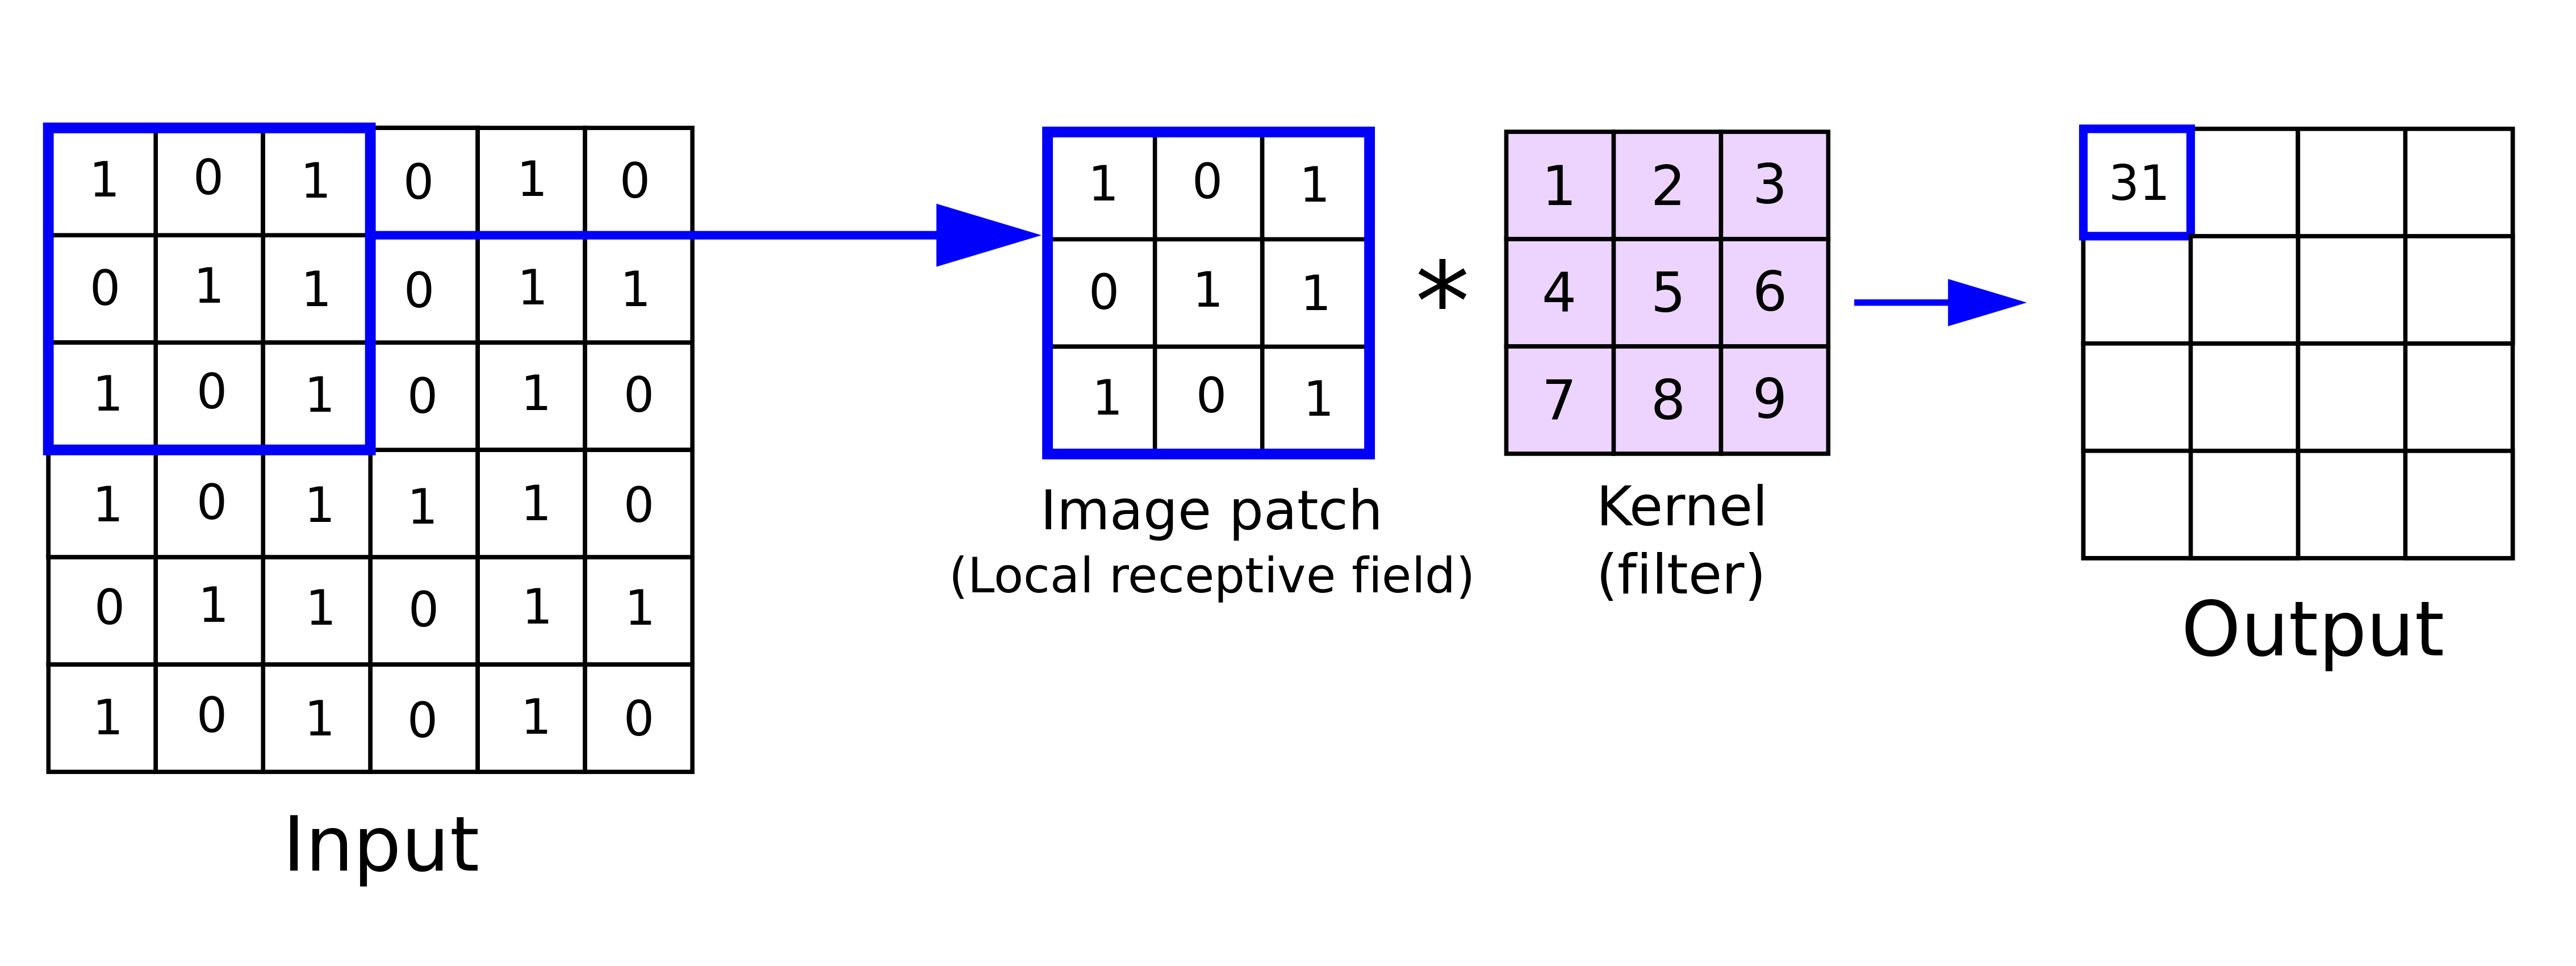
\includegraphics[width=120mm]{figures/convolution.png}
        \caption{Convolution matrix multiplication \cite{reynolds_anh_nodate}}
        \label{fnd:convolution}
\end{figure}

 Typically between subsequent convolutional layers, there are pooling layers. Pooling layers are used to reduce the spatial size of the feature maps produced by the convolutional layers. This helps to make the network more efficient by reducing the number of parameters that need to be learned, and can also help to prevent overfitting (where the network becomes too specialized to the training data).

The most common type of pooling layer is max pooling, which works by taking the maximum value of a set of adjacent pixels in the feature map. For example, a 2x2 max pooling layer would take the maximum value of each 2x2 patch of pixels in the feature map, resulting in a feature map that is half the size of the original. Other types of pooling layers include average pooling, which takes the average value of a set of adjacent pixels, and sum pooling, which takes the sum of the values in a set of adjacent pixels.

So the network is usually made of a stack of convolutional and pooling layers that extract and refine the features learned in the previous layers as shown in figure \ref{fnd:deep_cnn}. In this process the feature maps transition from representing lower-level features like lines into a more semantic representation like a shapes and objects in the scene.

\begin{figure}[H]
        \centering
        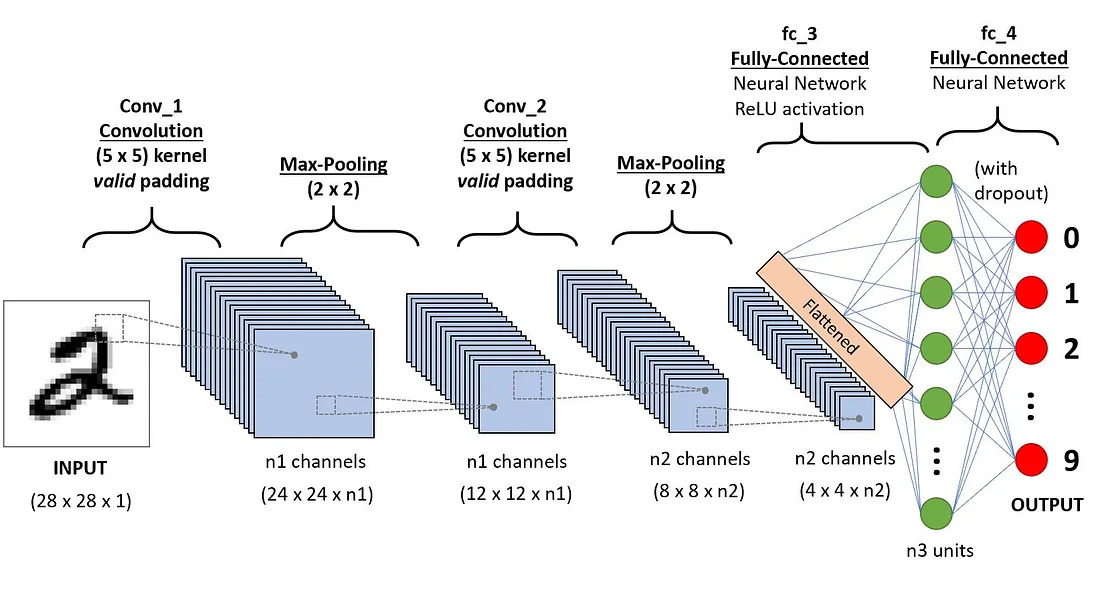
\includegraphics[width=120mm]{figures/deep_cnn.jpg}
        \caption{Deep CNN architecture \cite{saha_comprehensive_2022}}
        \label{fnd:deep_cnn}
\end{figure}

\subsubsection*{Overfitting}

But with the complexity introduced by deep CNNs, problems like overfitting arise. Overfitting is a common problem in machine learning, including neural networks, where a model is trained to fit the training data too closely, including the noise in the data, rather than generalizing to new, unseen data. This means that the model is essentially "memorizing" the training data rather than learning to make accurate predictions on new data.

In neural networks, overfitting can occur when the model is too complex, with too many layers and neurons, relative to the amount of training data available. This can cause the model to learn the noise in the data, rather than the underlying patterns and relationships that generalize to new data.

Overfitting can be detected by comparing the performance of the model on the training data to its performance on a separate validation set. If the model performs well on the training data but poorly on the validation set, it may be overfitting.

Several techniques can be used to prevent overfitting in machine learning. Some of the most commonly used techniques are:

\begin{itemize}
    \item Regularization: This involves adding a penalty term to the loss function, which discourages the model from overemphasizing any one input feature or from having large weights and biases. L1 and L2 regularization are two common types of regularization used in neural networks.
    \item Dropout: This involves randomly dropping out neurons during training, which reduces co-adaptation of neurons and encourages the model to learn more robust features.
    \item Early stopping: This involves stopping the training process before the model starts to overfit. This can be done by monitoring the performance of the model on a validation set and stopping training when the validation loss starts to increase.
    \item Batch normalization: This involves normalizing the inputs to each layer of the neural network, which reduces the internal covariate shift and makes the optimization process more stable.
    \item Data augmentation: This involves increasing the size of the training set by applying transformations to the data, such as rotation, scaling, or flipping.
    \item Ensembling: This involves combining multiple models to make predictions, which can reduce overfitting by averaging out the errors of individual models.
\end{itemize}

These techniques can be used individually or in combination to prevent overfitting and improve the generalization performance of a neural network.

\section{Text Localization Methods}

Text localization, also referred to as text detection, is the process of finding text in an image. The found text might have different fonts, colors, sizes, shapes, and partial occlusions. Text localization may also be considered a particular application of object detection methods.
The input is a whole image in which we want to find texts.

After the text has been located in the image, the output is a bounding box describing the location of the text. Bounding boxes consist of the center of the box and its corresponding width and height.

If the goal is not only to place a bounding box around the object but also to delineate the exact contour of the object of a certain class, i.e. we want to define which pixels belong to a certain class of objects then the problem becomes a semantic segmentation problem. If the goal is taken a step further and we want to differentiate between the pixels of each instance of each class of objects, then the problem is considered an instance segmentation problem.

This is a necessary step before running text recognition, as recognition methods usually work by transcribing a single word at a time and are typically more expensive to compute than text detection, as we will see later.

\subsection{Traditional Methods}
Traditional object detection methods were region proposal-based methods; the name originates from the way the algorithm works, which consists of five stages: a region proposal stage, a feature extraction stage, a judgment stage, an adjustment stage, and a suppression stage \cite{wang_object_2021}.

The region proposal stage proposes multiple regions in the image with a good chance of having an object inside of them called \gls{roi}. One of the widely used frameworks is the Viola-Jones algorithm \cite{viola_rapid_2001}. It uses the sliding window principle with HAAR filters set to generate the proposed \gls{roi}s.

In the feature extraction stage, a set of handcrafted filters are used to extract useful features about the \gls{roi}; some known techniques for using choosing robust filters include scale-invariant feature-transform (SIFT) \cite{lowe_object_1999} and histogram of oriented gradients (HOG)\cite{dalal_histograms_2005}. The result is a vector representing each feature's value in the \gls{roi} which can be used with classification methods like \gls{svm} to decide whether the given \gls{roi} contains some text. One such method that made use of \gls{svm} is Deformable Part Method 
(DPM)\cite{felzenszwalb_object_nodate}. It improves the Bounding Box's fit over the actual object inside the \gls{roi}.

After the fourth step, there might be multiple overlapping bounding boxes; as we are usually interested in only one, we need to filter the rest out based on some criteria like Non-Max-Suppression; For regions with a high overlap ratio which is calculated using \gls{iou} only those with the highest score from the \gls{svm} are left, and the rest is removed (suppressed).

\subsection{Machine Learning based methods}

 Although the main idea behind deep \gls{cnn}s was first introduced by Yann Lecun in 1998 \cite{lecun_gradient-based_1998}, they only became mainstream after the now famous AlexNet model was published in 2012 \cite{krizhevsky_imagenet_2012} which won the ImageNet competition. The AlexNet model influenced many models after it, some that used GPUs to accelerate learning and others that experimented with the influence of depth and recurrence on the overall performance.

 \subsubsection*{Two-Stage methods}

The \gls{rcnn} model \cite{girshick_rich_2014} model was one of the models built on the advancements made by AlexNet to improve object detection accuracy and speed. It has similar stages to traditional models, with the first stage being region proposal, then feature extraction, followed by a judgment stage. For the region proposal stage, it uses the selective search algorithm \cite{uijlings_selective_2013} to cluster regions/pixels with similar color, texture, and size and fill into blobs which are also aggregated into bigger chunks. In contrast to traditional methods (e.g. sliding-window) that result on average in $\sim100000$, this algorithm results in around $\sim2000$ candidate regions \cite{wang_object_2021} drastically improving performance. In the feature extraction stage, instead of using handcrafted filters, it uses a pre-trained AlexNet model to turn the proposed regions into vectors of feature values. The feature vectors are then processed by parallel \gls{svm}s and filtered using Non-Max-Suppression to get the final bounding boxes.

The different techniques used in the stages of \gls{rcnn} make it hard to train the whole model end-to-end. In addition, in the feature extraction stage, the \gls{cnn} has to run on every proposed region, even if it overlapped with another proposed region, which led to unnecessary repeated calculations.

Fast R-CNN \cite{girshick_fast_2015} solved the redundant computations problems by running the original image through several convolutional and pooling layers once and then projecting any given \gls{roi} onto the feature map. The projected feature map is then passed through a single layer \gls{sppn} to get a fixed-size feature vector. This output vector is then fed to a \gls{fcn}, which replaces the multiple \gls{svm}s in the normal R-CNN, enabling end-to-end training of the model.

Faster R-CNN \cite{ren_faster_2017} improved on Fast R-CNN by replacing the selective search algorithm with a \gls{rpn}; it runs on the feature map generated by the convolutional layers of R-CNN to propose \gls{roi}. This is implemented using an $n\times n$ and two $1\times 1$ convolutional layers. The center of the kernel in the $n \times n$ convolutional layer represents the center of multiple anchor boxes of different sizes and aspect ratios. The bounding boxes are then fed to the two $1\times 1$ layers, which give them a respective objectness score. This integration of the \gls{roi} proposal step allows it to be trained along with the rest of the network.

\label{maskrcnn}Mask R-CNN \cite{he_mask_2017} extends Faster R-CNN with a \gls{fcn} with a deconvolution layer to generate instance segmentation masks. The new \gls{fcn} runs parallel to the fully connected layers and yields a mask that assigns a class to each pixel in the image.

In Fast R-CNN, the \gls{rpn} runs only on the last feature map outputted by the backbone (e.g., AlexNet, ResNet, VGG-16...); the last feature map is a more semantically dense representation of the original image, but it has less of the details of the original. This lost information affects especially small objects in the picture; hence the object detection accuracy of fast R-CNN is usually worse for smaller objects. The \gls{fpn} method \cite{lin_feature_2017} remediates this problem by building a feature pyramid of the original image at different scales. This is done by combining feature maps from deeper layers in the backbone with the ones one level higher by upsampling them and then merging using some element-wise operation like addition; the resulting feature maps include both the semantic information from the deeper parts of the network and the details of the original, which improves the overall accuracy of the object detection and segmentation in the case of the Mask R-CNN.

\label{panet}\gls{panet} \cite{liu_path_2018} took this idea of feature pyramids a step further and added a bottom-up path connected in the reverse direction to the feature maps generated by \gls{fpn}, creating an easier way for the details from the original image to flow to the deeper-level feature maps. A given region proposal is then sampled from the feature pyramid and merged into a single region proposal using an adaptive feature pooling method.

\label{psenet}Other segmentation-based text detection algorithms include the \gls{psenet} model \cite{wang_shape_2019}, which is based on the \gls{fpn} architecture and a post-processing algorithm called "scale expansion algorithm". The input image is first passed through the ResNet model \cite{he_deep_2016}, the output of which is then augmented using the \gls{fpn} method to generate a feature pyramid; multiple segmentation masks are then generated based on the feature maps by passing them through two convolutional layers and an up-sampling layer. The scale expansion algorithm then takes these segmentation masks and expands the text regions until they include all the pixels belonging to a particular line of text.

\label{dbnet}\gls{dbnet} \cite{liao_real-time_2019} boosts a very similar structure to PSENet with a small change to how the binarization process works. In most segmentation-based object detection methods, the backbone and the neck of the network produce a probability map for the target class in the image, which is then binarized to produce the segmentation mask, which is later used to generate the object detection bounding boxes or polygons. This binarization process is quite often pretty simple and consists of comparing the probability of each pixel with a constant threshold set by the developer as a hyper-parameter; this can be expressed mathematically by
\begin{equation}
    B_{i,j} = 
    \begin{cases}
        1,& \text{if }_{i,j} P\geq threshold\\
        0,              & \text{otherwise}
    \end{cases}
\end{equation}
is not differentiable at the threshold value, and the derivative is $0$ otherwise, which means that it can't be optimized using back-propagation in \gls{sgd}. \gls{dbnet} proposed a "Differentiable Binarization" algorithm using a sigmoid function as an approximate step function which works well with back-propagation. By replacing the binarization function, the whole binarization process can now be trained along with the rest of the network to generate a dynamic threshold map that sets the threshold value per pixel instead of using a global constant, thus giving the network more flexibility to learn what should be considered as text and what not.

\label{dbnetpp}\gls{dbnetpp} \cite{liao_real-time_2023} the sequel of \gls{dbnet} optimizes the process of merging the different feature maps produced by the \gls{fpn}. In PSENet and \gls{dbnet}, the merging of the feature maps is a simple concatenation process; \gls{dbnetpp} improves this process by introducing an "Adaptive Scale Fusion" Network that adds an attention mechanism to the whole process. Attention mechanisms in machine learning are techniques that guide the focus of the network to a specific part of the image/object that's being processed to improve the performance of the task, somewhat similar to how the human perceptive system works; when understanding a scene, humans usually focus on certain key areas which explain the context and the main objects. The adaptive scale fusion model does a similar job by directing the focus of the network to the different scale features produced by the \gls{fpn} hence improving the detection of varying size texts in the image.

\label{fcenet}FourierNet, a.k.a FCENet \cite{riaz_fouriernet_2021} also uses segmentation to detect the text regions based on a ResNet \cite{he_deep_2016} + \gls{fpn} backbone followed by one classification and one regression head. In contrast to other models, FourierNet chooses to represent the text regions as coefficients for a Fourier series (hence the name) instead of a mask or a polygon. These coefficients can then be turned into a Polygon using the inverse fast Fourier transform. The size of the output vector determines the range of frequencies for the IFFT and thus determines the level of detail in the generated contour. The proposed representation is more compact than a polygon or mask representation, requiring less space.

 \subsubsection*{Single-stage methods}

But not all models were based on region proposals and FPNs, in 2016 Redmond et al. introduced the revolutionary \gls{yolo} object detection technique that found all objects in the scene using one forward pass through the convolutional layers achieving real-time detection speeds. The \gls{yolo} v1 model is based on the GoogleNet \cite{szegedy_going_2015} architecture which is a cascade of convolutional layers and max-pooling layers. It takes an input image of size $448\times448$ and divides it into $S\times S$ cells (typically $S$ is an odd number like $7$) and outputs $B$ bounding boxes for each cell. The bounding boxes contain $x$ and $y$ coordinates of the center of the bounding box relative to the edges of the current cell and the width and height of the bounding box and its confidence prediction. The results from all the cells are then passed to two fully connected layers that output the final class prediction for each cell. Because multiple bounding boxes from multiple cells might have the same class prediction and have a big overlap, all of the bounding boxes are passed through the \gls{nms} algorithm that returns the bounding boxes with the least amount of overlap and highest class confidence. Given two bounding boxes, \gls{nms} first measures the \gls{iou} between the two, and if it passes a chosen threshold then the bounding box with the smaller confidence gets discarded; this is then repeated until no more boxes have an IOU bigger than the threshold.

This architecture struggled with detecting objects of different sizes and generated only one class prediction per grid cell even if there were multiple objects in a given cell. These problems were alleviated by the introduction of YOLOv2 (YOLO-9000) in 2017 \cite{redmon_yolo9000_2017} which boosted a very similar structure to v1 but included many improvements. V2 switched from using GoogleNet to a ResNet backbone \cite{he_deep_2016} which allowed it to go deeper and learn more complex features. They dropped fully connected layers in the head and switched to using fully convolutional ones with anchor boxes. Anchor boxes are rectangles of pre-chosen width and height and they're used as a reference for the predicted bounding boxes. So the generated bounding boxes simply define a scaling factor of one of the anchor boxes. This helps the model recognize objects of different sizes and aspect ratios better as the anchor boxes can be chosen to be horizontal, vertical, big, and small. Multiple other changes were also made, like adding batch normalization, changing the reference for the bounding box center prediction, using hierarchal class classification, and multi-scale training. Overall, YOLO-9000 improved the performance and speed of the model.

YOLOv3 \cite{redmon_yolov3_2018} released in 2018 was an incremental improvement on v2 and improved the performance by switching to a different backbone called Darknet-53 and using multi-label instead of multi-class predictions. YOLOv4 \cite{wang_scaled-yolov4_2021} (2021) changed the backbone to the more powerful CSPDarknet53 network featuring their cross-stage partial connection blocks which similar to residual blocks help with the vanishing gradients problem. Also, the training was changed to use Self-Adversarial Training consisting of two stages; the first stage tries to remove the object to be recognized from the picture and the second stage tries to recognize the object that was removed by the first stage. YOLOv7 \cite{wang_yolov7_2022} released in 2022 changed the backbone another time to the Extended Efficient Layer Aggregation Network (E-ELAN). E-ELAN is a further development of the ELAN network released in 2020 and it puts heavy emphasis on being lightweight in order to run on edge devices like smartphones. ELAN uses a novel layer aggregation mechanism that combines the outputs of multiple layers in the network. This aggregation helps to maintain strong feature representations while reducing the number of parameters and computations required by the network. The architecture consists of several blocks, each of which contains multiple convolutional layers, batch normalization, and activation functions.

\section{Text Recognition Methods}
Text recognition is transcribing an image to machine-readable text such as ASCII.

Usually, run on an image containing a single word, text recognition methods work by transcribing the word character by character, which is mainly a classification task.
Classification methods try to find which set of categories -in this case, character class- a particular object or observation -in this case, an area of the image- belongs to.

As a classification task, text recognition methods work only for a particular set of characters that may or may not be shared between multiple languages. For example, the Latin alphabet is used by different languages; hence a non-dictionary-based text recognition method trained to recognize the Latin alphabet might be able to transcribe all those languages.
\subsection{Traditional Methods}
Optical character recognition methods first saw real-world use in the receiver address recognition for automatic mail distribution in the post office. Designed to recognize only specific text fonts, most recognition methods consisted of three main steps: regularization, segmentation, and recognition \cite{wang_object_2021}.

Images captured in the wild are usually imperfect and are plagued with problems like motion blur, perspective distortion, bad lighting, and noise. The Regularization step takes an input image with one or multiple of these problems and fixes them using a multitude of techniques. Blur and noise problems, for example, can be alleviated using deconvolution, while bad lighting caused by spectral reflections can be solved by combining two images with different light sources.

The segmentation step now takes the regularized image and segments it either by dividing it into subregions or based on some manually chosen features. It includes information about the sum of pixels in a particular column that surpasses a certain threshold, gradient information, or convex hull information.

Finally, these sub-regions with a letter each are fed into the recognition step to be transcribed into machine-readable text. The recognition methods evolved throughout the decades from recognizing only specific fonts to trainable systems that can identify new languages. The first systems used template-matching to transcribe the words, and in its simplest form, it's just a database of images and their corresponding letter; the new image is compared using pixel-wise difference against the list of templates, and it's matched with the closest one (i.e., the template with the slightest difference). That has been later improved using deformable templates, which, as the name suggests, are deformed during inference to match the sample image to fix the shortcomings of fixed templates like sensitivity to small rotations and skew. Though it worked for very constrained use cases, template matching wasn't reliable enough and was quickly surpassed by probabilistic models like perceptrons, \gls{svm}s, and hidden Markov models. \gls{svm}s learn to differentiate between objects (in this case, characters) based on only a subset of key features, which are called support vectors; still used to this day, they're sometimes good and faster alternatives to deep neural networks when it comes to specific classification tasks. Hidden Markov models, a particular case of Markov models, are probabilistic models built on top of the bayesian theorem for conditional probabilities and are suited for time-series forecast, as this is the case for forecasting the next letter in a word.

\subsection{Machine Learning based methods}

\subsubsection*{Deep Convolutional Neural Networks}

Text recognition is mainly a classification task, i.e., deciding which class an object belongs to; this is due to how most recognition methods work, which is by going through the subregions of an image and trying to assign the object contained within it to a particular class of objects, and in the case of text recognition the classes are the letters in the chosen character set.

As with text localization methods, \gls{cnn}s and mainly deep \gls{cnn}s have proven well suited for object classification tasks. The architecture of a typical deep \gls{cnn} contains multiple sets of convolutional layers followed by pooling layers; the convolutional layers' main task is feature extraction, and they're made of kernels (matrices) which get multiplied element-wise by their input matrices and after training their values get updated in such a way that they specialize in recognizing certain features in the input for example edges, vertical and horizontal lines or round shapes. The pooling layers take an input matrix and convolve over it to reduce the size of the image as it goes deeper through the network by taking only the average or the maximum of a small window as the output, and this has functional and performance reasons; functionally it forces the network to aggregate lower-level features like lines and edges into more semantically relevant features like shapes the deeper they are in the network, and it increases the performance as it requires less memory to store all the layers and hence allows for deeper networks. So given an input image, a deep \gls{cnn} encodes the image's content into a small vector representation which can then be used as input for a classification algorithm like \gls{svm} to decide what the actual content of the image is.

Deep \gls{cnn}s can't be applied directly to a text recognition task because of two problems. First, learning to recognize complete words and their variations is infeasible and impractical, it's infeasible because we would have to get a dataset with all the possible words in a language with variations in fonts, size, etc. and the training would take too long because the softmax layer would have to calculate the probability of every single possible word. Second, it's impractical because it would mean that the model will only be able to recognize words in our dataset, meaning that we would have to get training data for every new word and train the model to recognize that particular word. That's why most models are trained to recognize only the characters in an alphabet (character set) and not complete words. That poses another challenge, given that the bounding boxes outputted by the text detection algorithms usually contain whole words and not only characters, making it impossible to use the character-level classification models on the image to recognize the word directly, but because \gls{cnn}s slide over the whole image, in the final output vector each column can be mapped to a specific column in the original image from left to right; hence the final output represents the encoding of different segments of the image. These encodings can then be passed to a sequence-to-sequence model or a classifier.

\subsubsection*{Recurrent Neural Networks}

Sequence-to-sequence models are models that take, as the name suggests, a sequence of data and generate a new sequence as output as shown in figure \ref{fnd:seq2seq_rnn}; \gls{rnn}s are such models. They are made of memory cells, and they're somewhat similar to perceptrons in function; they take in an input vector and multiply it with a weights vector, but RNN blocks also take in a "memory" (hidden state) vector and also multiply it with a weights vector and then added it the input vector; and they output two vectors, one being the actual output and the second is a hidden state. When the input hidden state vector is the vector outputted from the previous RNN block, the architecture becomes a chain with one block influencing the next one; using this mechanism, \gls{rnn}s implement the concept of memory (history) and allow previous inputs to influence the output for the current one.

\begin{figure}[H]
        \centering
        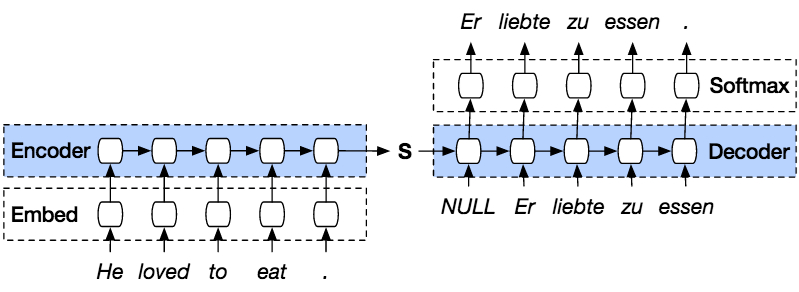
\includegraphics[width=120mm]{figures/seq2seq_rnn.jpg}
        \caption{Sequence-to-sequence RNN \cite{johnson_seq2seq_2020}}
        \label{fnd:seq2seq_rnn}
\end{figure}

They can be configured and used in different ways; for example, if the goal is to use it as a sequence-to-sequence model, then it can be built in an encoder-decoder architecture with the encoder being a chain of RNN blocks and the hidden state of one block being fed to the hidden state of the next one and all the outputs ignored, the final hidden state outputted after the last token in the sequence is an encoding of the whole input sequence; this encoding is then passed to the decoder as the hidden state of the first block with a corresponding Start Of Sentence (SOS) token as input, then the output of one block can be fed as input for the next block until a chosen End Of Sentence (EOS) token is outputted; the resulting sequence is the output sentence.
Normal RNN blocks suffer from two main problems, exploding and vanishing gradients problem; while training the network, \gls{sgd} fails to optimize the weights, because the gradients calculated with back-propagation are either too big (exploding) or too small (vanishing), this is due to the fact that the hidden state gets multiplied in every block, in the case where the weights are smaller than zero then it becomes close to zero and in the case, it's bigger than one it becomes very big very quickly. \gls{lstm} cells were introduced to solve this problem, they have two types of memory, short-term and long-term where the long-term memory gets updated in every cell and isn't directly multiplied by weights instead a percentage of the old value is retained (remembered) and a new value (memory) is added to it.

If the input sequence for the encoder is made of the columns outputted by the \gls{cnn} from the previous step, then the encoder's output will be an encoding of the word contained in the image, which the decoder will then translate to machine-readable characters, and that's how the \gls{crnn} model \cite{shi_end--end_2017} works.

\label{sar}The \gls{sar} model \cite{li_show_2019} has the same architecture as \gls{crnn} but adds an extra attention module that helps with recognizing irregularly-shaped text. The attention module is part of the decoder and for each block, it takes the outputted hidden state and the feature maps generated by the encoder and calculates an attention vector which is then appended to the current output and multiplied with a weights matrix to get the final output (character).

\subsubsection*{Transformers}

Although \gls{rnn}s are flexible and good at understanding sequential data like languages (words), they have some problems that limit their use in real-world situations; they need to process data sequentially (one element after the other), making them relatively slow both when training and when running inference, and this inherent inability to process data in parallel means that these models can't make use of hardware acceleration.

In 2017, AI researchers at Google published a paper named \\ \mbox{"Attention Is All You Need"} \cite{vaswani_attention_2017} that aimed to solve the shortcomings of \gls{rnn}s; the authors chose to name their model the "transformer" and it has proven to be useful for both natural language understanding (NLU) and computer vision tasks. Transformers are also sequence-to-sequence models and have an encoder-decoder architecture, meaning that the encoder takes in an input sequence and encodes to a vector representation which is then given to the decoder to translate into an output sequence. Most building blocks used in transformers are the usual ones used in most models, like linear layers, activation layers, and skip connections, but the paper introduced some novel building blocks like \gls{mha} and positional encodings. The architecture of the model is represented in figure \ref{meth:transformer_architecture}

Position embeddings are what allow parallelism when using transformers. To understand what position embeddings are, one must first understand what embeddings are; as most models can't work directly with textual data and only understand vectors, the words in a given sentence need to be transformed (embedded) into n-dimensional vectors that represent the meaning of the word with n being the embedding size; these representations are learned using unsupervised learning methods like masked token prediction which simply asks a network to guess what a hidden word in a sentence is. After training, vectors of words with similar meanings like "game" and "play" end up clustered together in the n-dimensional space. Positional embeddings simply add a vector of a similar size to the embeddings of each word in the sentence unique to its position in the input sequence (sentence); so the resulting vector not only encodes the meaning of the word but also its position in the sentence allowing the whole sentence to be fed in parallel to the model.

\begin{figure}[H]
        \centering
        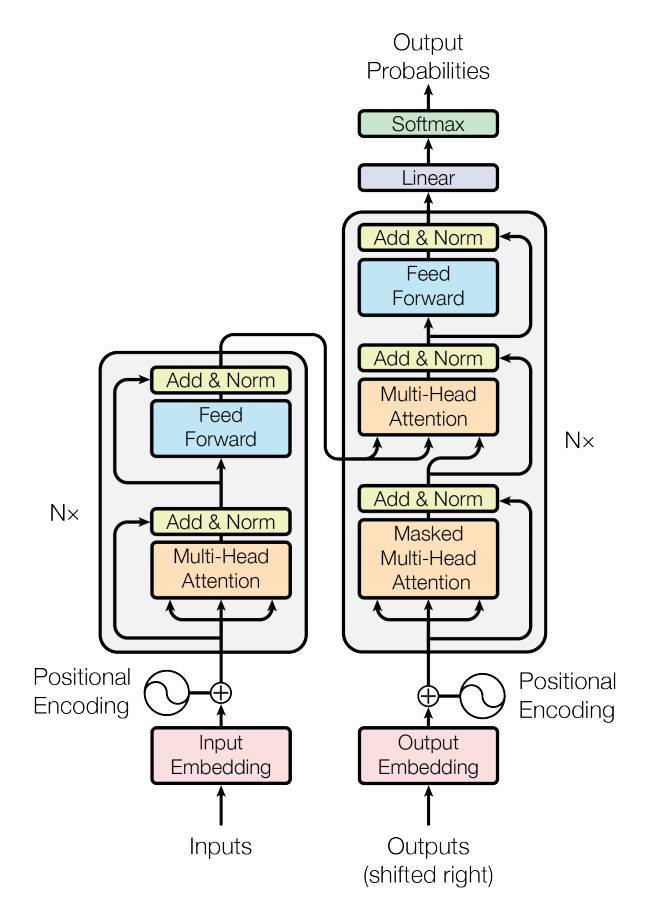
\includegraphics[height=100mm]{figures/transformer_architecture.jpg}
        \caption{Transformer Architecture\cite{noauthor_language_nodate}}
        \label{meth:transformer_architecture}
\end{figure}

The \gls{mha} block is the most crucial part of the transformer model, and it implements the concept of self-attention; it takes in three vectors named Key, Query, and Value as input, and it encodes how important (relevant) the elements in the value vector are based on the similarity between the key and the query; the similarity between the key and the query is determined using cosine similarity which results in an attention mask that is then multiplied with the value vector resulting in value vector with importance values encoded in it; this process is inspired by how content retrieval system work, given a user's query they go through the keys in their database and rank value based on their relevance. In the encoder part of the transformer, the key, query, and value matrices are all the same matrix, which contains the positional embedding of the words in the input sentence; the \gls{mha} then proceeds to calculate how similar the key and query matrices, which are the words in the sentence are similar to each other and then updates their value based on the attention mask, thus making the words in the sentence look at other words in the sentence and determining how relevant they're to them; hence it's called self-attention. The output of the MHA block goes through a feed-forward block and a skip connection creating a logical compound block that can be stacked to generate the encoder part of the transformer. The decoder of a transformer consists of two stacked MHA modules followed by a fully connected layer and a softmax layer; the first MHA block takes in the previously generated sequence, so the model can pay attention to what it has already generated while the second MHA block takes in the output of the first block as the value matrix and the encoder's output as key and query to relate what it already generated to the input sequence. This architecture has proven to be highly versatile at natural language understanding tasks, like question-answering and neural machine translation, but with some minor additions, transformers can also be used in computer vision tasks like text recognition; the main addition is usually an image embedding layer before the position encodings, this is done because images can be pretty complex and a more simplified vector representation of the different regions of any image is needed, an excellent tool for the job is \gls{cnn}s. So the image is first fed through a \gls{cnn}, and the output is passed to the transformer. \label{nrtr}\mbox{\gls{nrtr}} \cite{sheng_nrtr_2019} is one of the model that has this architecture.

\label{satrn}\gls{satrn} \cite{lee_recognizing_2020} is a text recognition model with a similar architecture to the one described with minor changes to improve the recognition performance on irregularly shaped text. The first change is adding two scalars to the position embedding layer, which are generated dynamically based on the feature maps outputted by the shallow \gls{cnn}; these two scalars make the positional embeddings represent horizontal and vertical text better. The second change is to the feed-forward layers after the \gls{mha} block, making the network focus more on features that are close to each other.

\label{master}\gls{master}The encoder-decoder architecture of transformers is extremely versatile but the encoder and the decoder are also quite useful on their own and can be combined with different encoders and decoders. \gls{master} \cite{lu_master_2021} used the normal transformer decoder but replaced the encoder; the encoder is based on the global context aggregation block introduced in GCNet \cite{cao_gcnet_2019}. The global context block provides an attention mechanism that encodes the global image context to help with the task. In contrast to \gls{cnn}s which focus on local features, the global context block helps the encoder focus on different objects in the image; this is done by running the feature maps through a \gls{sen} based network, which generates attention masks that are then added to the original feature maps.

Text recognition is mainly a computer vision task, meaning the recognition of the word in the image is based only on pixel values. Still, sometimes the image might be blurry, too small, or occluded, as is the case when a professor's hand covers part of a word while writing on the board. In such cases, though impossible to say for a certain what the unreadable letters are, a language model might help to guess what the word is. A language model is, is model that was trained to learn the probabilities that exist in a language, like the probability of a word/character given the probabilities of the words/characters preceding or surrounding it. When a letter can't be determined using vision-only methods (described above) or the recognized character's confidence doesn't pass a certain threshold, it might be helpful to try to guess what that character is using a language model. This can be done either while running the inference by conditioning each recognized character on the characters recognized before it, like in an autoregressive model, or as a post-processing step by refining the recognized word iteratively. Most text recognition methods use an external language model that is mostly independent of the vision task and can be trained separately; some models use only character-level probabilities while others may also use word probabilities, so words that are used more frequently in a language are preferred to those that are less frequent. On the other hand, some models integrate the language model into the sequence-to-sequence model and make the character correction part of the decoding process.

\label{parseq}\gls{parseq} \cite{bautista_scene_2022} is one such model based on transformers a and an integrated language model. Other computer vision models that use transformers usually make use of \gls{cnn} before feeding the input image into the transformer's encoder, but \gls{parseq} uses \gls{vit} \cite{dosovitskiy_image_2021}, which is a direct application of transformers on images, it segments the input image into regions of equal size, flattens then embeds them. The innovation made by \gls{parseq} lies in the decoder that learns the language model while training. The decoder is not fed the produced sequence as a key, query, and value vector like in the standard transformer decoder; instead, the query is replaced with position queries that tell the decoder which part of the output sequence we want to generate, hence allowing the model to generate the output sequence in random order, not necessarily left-to-right or right-to-left. The decoder is trained using permutated attention masks, which makes it non-autoregressive, i.e., independent of the order of decoded characters. When running inference, the position queries and the attention masks combined can generate different modes of operation; by making the model decode the input sequence character by character and only pay attention to the characters to the left, it will work as an autoregressive model; on the other side, by making the model decode the characters in random order while paying attention to the whole outputted sequence, it can function as an iterative refinement model.

\section{OCR challenges} \label{ch:foundations:ocr_challenges}

\subsubsection*{Related to performance}

Transcribing text in videos goes beyond simple text localization and recognition; for example, videos are just a set of frames (images), and a typical one-hour thirty-minute long video recorded at 30 \gls{fps} contains $90 * 60 * 30 = 162000$ Frames that need to be processed individually. If processing one frame takes 100ms, this video will take four hours and thirty minutes, quickly becoming impractical when processing hundreds of lectures per day. Therefore, techniques like subsampling or distinct frame detection might be necessary to achieve practical processing speed. In subsampling, only a subset of the video frames are processed, and they're chosen by picking every nth frame or selecting a random frame every nth second; this makes sense for videos because usually there isn't that much change between two successive frames in a video, which were shot with less than 33ms time in between. While subsampling selects frames based on a fixed time period between them, distinct frame detection tries to filter the video and find the unique/distinct frames based on a certain difference threshold, i.e. given a set of $n$ images, find the subset of $i \leq n $ images which best represent the whole set. Distinct frame detection task falls under the category of video summarization and in recent years, as is the case with other computer vision tasks, it has seen a shift towards machine learning-based methods; most of these methods like DSNet \cite{zhu_dsnet_2021} and the one proposed in \cite{apostolidis_combining_2021} work by embedding the individual frames, i.e. computing a feature vector of each frame using \gls{cnn}s and then comparing the difference score between these vectors. The method proposed in this paper \cite{zhu_relational_2022}, makes use of \gls{rpn}s to detect objects in the scene and then tracks those objects across time and space; the distinct frames are then chosen based on the changes to the object graph. Machine learning-based video summarization techniques are usually compute-intensive and are not fast enough to be used as a preprocessing step to the main object detection task. This comes as a trade-off between speed and accuracy when used in a video processing pipeline; if the time saved by summarizing the video is less than the actual time it would take to run text detection and recognition on all the frames, then it becomes unnecessary. 

\subsubsection*{Related to variations in text}

Other challenges encountered while transcribing text from images are related to the \gls{ocr} task, as reading text can be challenging even for humans. This is caused by the fact that text can vary significantly based on whether it's typeset or hand-written and based on the person who wrote it. In contrast to typeset text that has only a somewhat limited number of fonts, hand-written text varies enough from person to person to be used to identify people based on their signature or determine their personality, like in the field of graphology.

The challenges posed by the variations in text are only compounded when trying to recognize text across multiple languages. According to Ethnologue, a language reference published by the Summer Institute of Linguistics there are 7151 spoken languages worldwide at the time of writing \cite{noauthor_how_2016}; most of them have unique character sets, some of these languages are written left-to-right, others right-to-left, some are written with separated letters, others with linked letters, and some are not even written. So trying to develop a single method to recognize different languages quickly becomes a daunting task even for the most advanced machine learning methods, especially when taking into consideration that some models integrate a language model in their recognition process and are therefore tailored to a specific language or only a set of languages.

\subsubsection*{Related to the methods}

In addition to challenges inherent to the \gls{ocr} task, some problems arise from the text localization and recognition methods themselves; one of these problems originates from the way the \gls{ocr} pipeline is constructed. As described earlier, to transcribe text found in images, we start by first detecting text in images by putting a bound box around it, and this is usually done word-wise; that is, every word in the image gets its own bounding box. It's generally necessary to do it word by word because of multiple reasons, including but not limited to the inability of some text recognition methods to read sentences as they were trained to recognize only words, the scarcity of text detection datasets that contain word-by-word segmentation, and it makes the recognition task after it easier. But this word-level segmentation causes a slight problem down the line if we wish to reconstruct the original sentences from the individual recognized words; this may be sought after to run some language model on the output instead of treating it as a bag-of-words. There hasn't been much research done on this topic, but a simple approach like stitching boxes based on their horizontal distance works in practice.

\subsubsection*{Related to recognition errors}

One further problem we might face when doing \gls{ocr} is the erroneous output of text detection or recognition models; even state-of-the-art techniques still make errors. In the case of text detection models, the text might not get detected or partially detected, leading to either non-transcribed or erroneously recognized text. Though detection problems might be hard to fix without completely changing the methods or retraining the model, text recognition problems might be remediated in post-processing. The same techniques used for this task are the ones used for misspelling correction in search engines, and there are two general classifications, either context-based or context-free error correction.

Context-free error correction is the easiest to understand and is probably what comes to mind when thinking of context-free error correction, and it's based on detecting \gls{oov} words. Given a dictionary (a list of words), an \gls{oov} word is a word that is not included in the list; for example, if the word "history" was incorrectly transcribed as "heestory", it will be flagged as a misspelling because it won't be found in the dictionary. The correction then works by finding the word in our dictionary with the shortest normalized edit distance to the misspelled word. The normalized edit distance \cite{yujian_normalized_2007} counts the number of one-letter insertions, deletions, and substitutions necessary to transform one string to another. An obvious limitation of this technique is the dictionary size and the different languages; creating a dictionary with all the valid words in a language is first infeasible as it would be huge and make the search for the corrected word slow, but it would also have to be updated regularly as new words are added to the language, added to that a dictionary should be created for different languages; that aside different, some words might be invalid in some languages but valid in others, meaning that we should also somehow detect the language of the text.

Context-based error correction is a bit more complex and employs different language analysis techniques ranging from grammatical analysis to a state-of-the-art language model. In contrast to context-free error correction, context-based error correction takes in a collection of words, usually arranged in a sentence, and determines whether the sentence is grammatically correct and even if it makes sense. Given that the context-sensitive error correction requires whole sentences instead of individual words, it's necessary to run the bounding-box stitching before running this step to form sentences from the individually recognized words. 
